\chapter{Parallelization of Regression Test Selection }
\label{sec:tldr}

In this chapter, we propose a novel, method-level, and static RTS tool, TLDR. We discuss how TLDR compensates the computational expense of finer-granularity change impact analysis by the application of parallelism. We then compare TLDR with other contemporary RTS tools through a synthetic example. 

\section{Concept}
We saw in chapter \ref{sec:background} that properties of RTS tool have a varying degree of performance implications. Table \ref{comparison} shows how each category of RTS tools varies in terms of precision, test selection time, and test execution time. As we can see, finer granular RTS tools have shorter test execution time because they select fewer tests. However, they incur large test selection time because change impact analysis in finer granularity is more expensive. Again, Static RTS tools have shorter test selection time, thus have shorter end-to-end time. Therefore, an efficient RTS tool that incurs lesser end-to-end time should be static. Moreover, it should combine the benefits of finer- and coarser-granularity RTS tools. As mentioned earlier, a finer granularity RTS tool incurs more test selection time. In this thesis, we explore the application of parallelism in the change impact analysis technique of a finer-granularity RTS tool to reduce the test selection time as well which will, in turn, reduce the end-to-end time. Therefore, we design TLDR, a method-level and static RTS tool that leverages an efficient and parallel \textit{pipe-and-filter} architecture~\cite{gokhale2006reliability, philipps1999refinement} along with a set of in-memory inverted and forward indices. 

\begin{table}[b]
\centering
  \caption{Categorization of RTS Techniques}
  \label{comparison}
  \resizebox{\columnwidth}{!}{%
    \begin{tabular}{|c|c|c|c|c|}
        \hline
    {\textbf{Property}} &  \textbf{Category} &  \textbf{Precision} & \textbf{Test Selection} & \textbf{Test Execution}\\
     &  &   & \textbf{Time} & \textbf{Time} \\
    \hline
    
    Granularity of  & Package & Very Imprecise & Small & Very Large \\
    Test Selection & Class &  Imprecise & Moderate & Large \\
     & Member &  Precise & Large & Small \\
    
    \hline
    
     & File &  Very Imprecise & Small & Very Large \\
    Granularity of  & Class &  Imprecise & Moderate & Large \\
    Change Analysis & Member & Precise & Large & Small \\
     & Statement & Very Precise & Very Large & Very Small \\
    
    \hline
    
    Dependency  & Static &  NA & Small & NA \\
    Collection & Dynamic &  NA & Large & NA \\
    
    \hline
    \end{tabular}%
    }
\end{table}%


Figure \ref{fig:sub1} shows the pipeline of a sequential RTS tool which includes four modules, namely, Change Analysis, Dependency Graph Generation, Change Impact Analysis, and Source to Test Map. In contemporary RTS tools, these phases are completed sequentially~\cite{ekstazi, starts, hyrts, faulttracer}. A key observation is these modules are partially independent for each class. For example, while we are analyzing recent changes in one class, we can analyze another class parallelly in the pipeline. Dependency graph construction must be synchronized among the classes as they are interdependent. However, after the dependency graph has been constructed, change impact analysis and source to test map are independent steps for each class. Therefore, given appropriate synchronization, we can employ multiple worker threads among each module and dramatically reduce the throughput of the pipeline. The core concept of TLDR is based on this parallel pipe-and-filter architecture. It parallelly passes each class of the project in the pipeline. In each module, a worker thread consumes the outputs of the preceding module. The worker threads that are not currently busy consume the outputs from a blocking queue. Ultimately the pipeline outputs a set of tests. We will discuss the design and implementation of TLDR in chapter \ref{sec:Implementation}.   

\begin{figure}[htb]
    \centering
    \begin{subfigure}[b]{\textwidth}
    \label{fig:sub1}
        \centering
        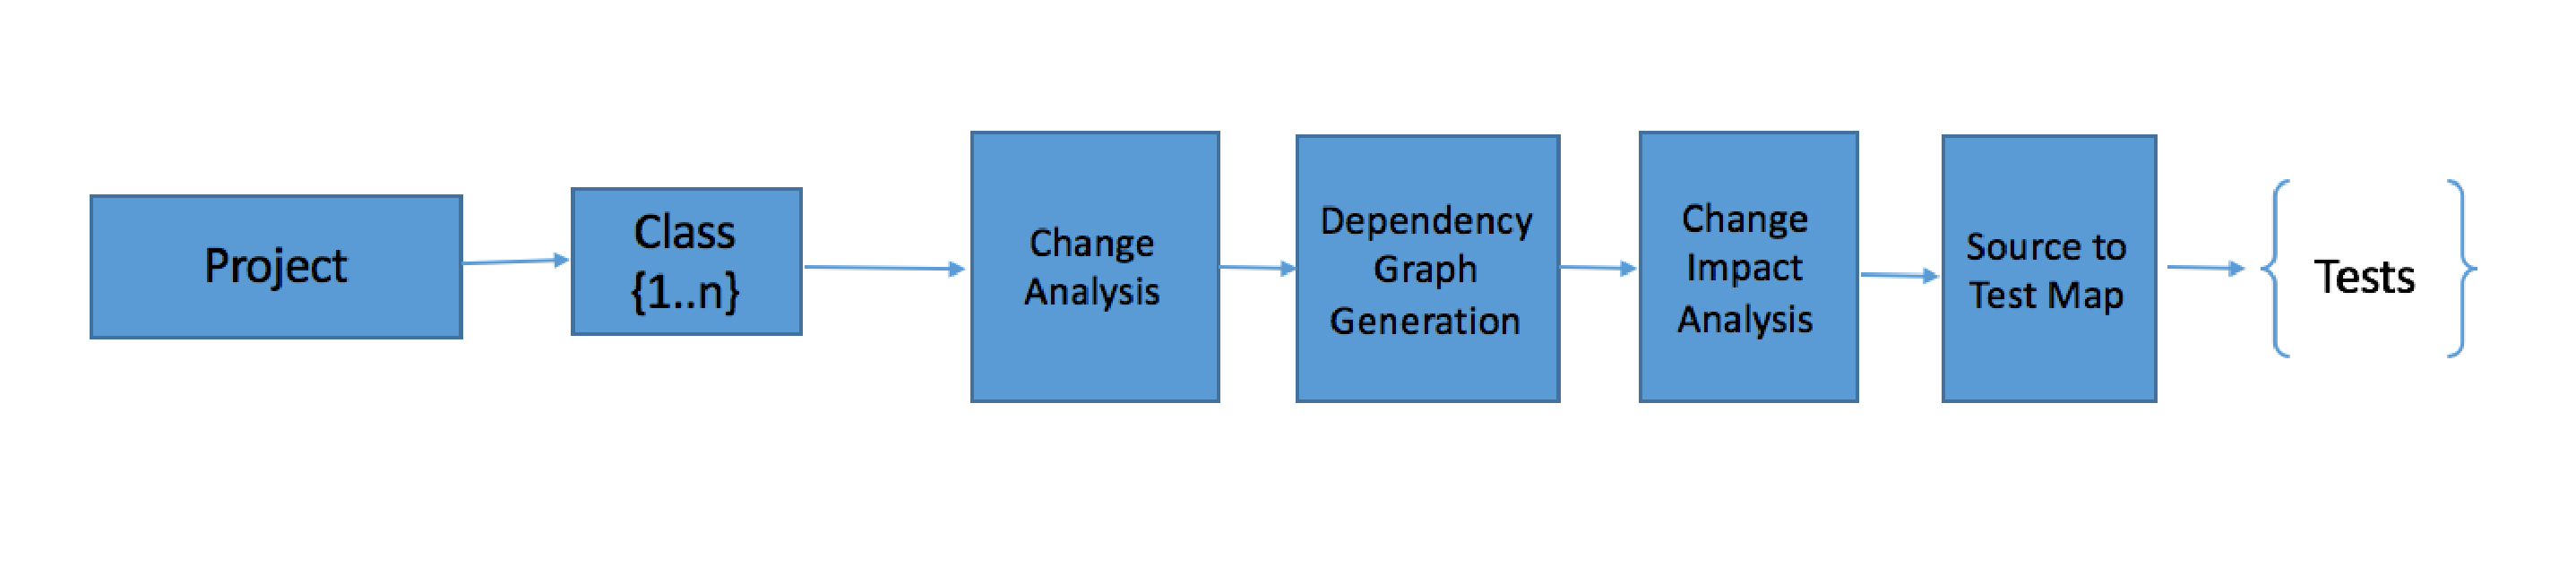
\includegraphics[width=0.99\linewidth]{pipe_1}%
        \hfill
        \caption{Sequential RTS pipeline}
    \end{subfigure}
    \vskip\baselineskip
    \begin{subfigure}[b]{\textwidth}
    \label{fig:sub2}
        \centering
        \includegraphics[width=0.99\linewidth]{pipe_2}%
        \hfill
        \caption{Parallel RTS pipeline}
    \end{subfigure}
    \caption{Generic pipeline of regression test selection.}
\end{figure}


\section{Example}
Table~\ref{comparison} summarizes the similarities and differences among four recent techniques, as well as our own, i.e., TLDR. What follows is an explanation of this table, followed by one concrete example of how three of these tools behave in the presence of a given change.

\begin{table}[b]
\centering
  \caption{Categorization of RTS Tools}
  \label{comparisontools}
  \resizebox{\columnwidth}{!}{%
    \begin{tabular}{|l|c|c|c|}
        \hline
    {\textbf{Technique}} &  \textbf{Granularity of} &  \textbf{Granularity of} &  \textbf{Dependency}\\
                         & \textbf{Test Selection} & \textbf{Change Analysis} &  \textbf{Collection} \\
    \hline
    \textbf{Ekstazi} \cite{ekstazi} & Class & File & Dynamic \\
    \textbf{STARTS} \cite{starts} & Class & Class & Static \\
    \textbf{HyRTS} \cite{hyrts} & Class/Method & Class/Method & Static+Dynamic\\
    \textbf{FaultTracer} \cite{faulttracer} & Method & Statement & Dynamic \\
    \textbf{TLDR } & Method & Member & Static \\
    \hline
    \end{tabular}%
    }
\end{table}%

Below, we explain the functionality of TLDR compared Ekstazi, STARTS, and HyRTS to illustrate how these three approaches differ along the dimensions of Table~\ref{comparison}. Table~\ref{example} shows an example Java project. Column \textit{Source} shows the source code and column \textit{Test} shows the test suite of the project. For each method in the source code, there is a test method in the test suite. Class \texttt{A} is extended by classes \texttt{B, D} and class \texttt{B} is extended by class \texttt{C}. Each of the sub-classes overrides method \texttt{A.f2}. Method \texttt{A.f1} is overridden by \texttt{C} and \texttt{D}. 

\begin{table*}
{\fontsize{12pt}{12pt}\selectfont
\centering
\caption{An Example Java Project}
\begin{tabular}{|p{0.5\linewidth}|p{0.5\linewidth}|}
\hline
\textbf{Source} & \textbf{Tests}  \\
\hline
\begin{lstlisting} [caption={}]
class A {
  String f1() { return new B().m1() + "a";}
  String f2() { return "a1";}
}
class B extends A {
  String m1() { return "b";}
  String f2() { return "b1";}
}
class C extends B {
  String f1(){ return super.f1() + "c";}
  String f2(){ return "c";}
}
class D extends A {
  String f1(){ return "d";}
  String f2(){ return "d";}
}
\end{lstlisting}

& 
\begin{lstlisting} [caption={}]
class TestA {
    A obj = new A();
    void tF1(){ assert(obj.f1() != null);}
    void tF2(){assert(obj.f2() != null);}}
class TestB {
    B obj = new B();
    void tM1(){assert(obj.m1() != null);} 
    void tf2(){assert(obj.f2() != null);}}
class TestC {
    C obj = new C();
    void tF1(){assert(obj.f1() != null);}
    void tF2(){assert(obj.f2() != null);} 
class TestD {
    A obj = new D(); // <--- note the declaration as A
    void tF1(){assert(obj.f1() != null);}
    void tF2(){assert(obj.f2() != null);}
\end{lstlisting}
\\
\hline
\end{tabular}
\label{example}
}
\end{table*}

The test selection sets when method \texttt{B.m1} changes are: 
\begin{itemize}
	\item Ekstazi: all test methods in \texttt{TestA, TestB}, and \texttt{TestC} -- 6 tests.
	
	\item STARTS: all test methods in \texttt{TestA, TestB, TestC}, and \texttt{TestD} -- 8 tests.
	
	\item HyRTS: test methods \texttt{TestB.tM1, TestA.tF1, TestC.tF1} -- 3 tests.
	
	\item TLDR: test methods that reach, or might reach, \texttt{B.m1}, specifically \texttt{TestB.tM1, TestA.tF1, TestC.tF1}, and \texttt{D.tF1} -- 4 tests.
\end{itemize}

Both Ekstazi and STARTS select tests at class level, so if any one test method needs to be retested, the entire class where that method is declared will be retested. TLDR selects tests at individual method level, so it can be more precise, as this example shows -- 4 test methods instead of 6 (Ekstazi) or 8 (STARTS). However, since this is an atomic change within the class, HyRTS only selects 3 methods. STARTS and TLDR use static analysis for tracking dependencies, while Ekstazi and HyRTS use dynamic analysis. Therefore, Ekstazi and HyRTS are more precise with respect to inheritance and method overriding. Let's look at the consequences of static vs. dynamic analysis for the test method \texttt{TestD.tF1}. That method instantiates a \texttt{D} object, but statically declares it as type \texttt{A}. Being an instance of \texttt{D}, and given that \texttt{D} overrides \texttt{A.f1}, the test method \texttt{TestD.tF1} does not need to be selected when \texttt{A.f1} changes. In this case, Ekstazi is able to identify that the \texttt{A}-object created in \texttt{TestD.tF1} is an instance of subclass \texttt{D}, while both STARTS and TLDR are unable to do so. 

Now let us consider another scenario where \texttt{Class D} is made to extend \texttt{Class C} but no method is changed. The test selection sets for this change are: 
\begin{itemize}
	\item Ekstazi: all test methods in \texttt{TestD} -- 2 tests.
	
	\item STARTS: all test methods in \texttt{TestA, TestD}, and \texttt{TestD} -- 4 tests.
	
	\item HyRTS: test methods \texttt{TestD} -- 2 tests.
	
	\item TLDR: No test method is selected -- 0 tests.
\end{itemize}

Even if no method was changed, \texttt{ClassD} will have different checksum, therefore, Ekstazi will select \texttt{TestD} and STARTS will select \texttt{TestA, TestD}. HyRTS considers class hierarchy change as class header change, thus it will perform file-level analysis and test selection. Therefore, it will select \texttt{TestD}. However, TLDR detects that even though the class hierarchy has been modified, no method was updated. Therefore, it will not select any test method. 